\section{Results}\label{sec:results}

In the following, the concrete implementation of the described models in \autoref{sec:methods} and the resulting results will be presented. The focus of the elaborations are the major findings of the work of Tran and Yates, accordingly not all results are listed herein. Details can be studied in the paper by Tran and Yates \cite{tran2022dense}.

\subsection{Experimental Setup}

Tran and Yates implemented their models in a TensorFlow (Abadi et al. \cite{abadi2016tensorflow}) setup: For the pretrained language model, they chose a distilled BERT (Sanh et al. \cite{sanh2019distilbert}), fine-tuned using TAS BERT approach (Hofst{\"a}tter et al. \cite{tasbert}), as described in \autoref{subsec:general_model}. Further, to determine the embeddings, Tran and Yates used Dexter (Ceccarelli et al. \cite{ceccarelli2013dexter}) and Wikipedia2Vec (Yamada et. al \cite{yamada2018wikipedia2vec}), as described in \autoref{subsec:entity_embeddings}. 

Training was done using pairwise hinge loss on four Quadro RTX 8000 GPUs in parallel on 300,000 training samples of the MS MARCO dataset (Nguyen et al. \cite{nguyen2016ms}). For the two models that allow indexing, i.e. EVA Single and EVA Multi (see \autoref{subsec:models}), the end-trained model was used to index embeddings for documents.

Evaluation was performed on 7,127 test samples from the MS Marco dataset and the datasets TREC Deep Learning (DL) Track 2019 (MacAvaney et al. \cite{trec_dl_2019}), TREC DL 2020 (MacAvaney et al. \cite{trec_dl_2020}), TREC DL HARD (Yates et al. \cite{dl_hard}). Evaluation metrics were chosen to be nDCG@10, MRR@10, MAP@1000.

Tran and Yates compared their own models EVA Single, EVA Single-QA and EVA Multi (see \autoref{subsec:models}), each with and without KNRM signal (see \autoref{subsec:knrm}), against different baselines:

\begin{itemize}
    \item BM25: The most prominent example of exact matching paradigm, using sparse representations (Robertson et al. \cite{BM25})
    \item TAS BERT: Fine-tuned BERT model using topic-aware sampling strategy as described in \autoref{subsec:general_model}.
    \item ANCE: A state-of-the-art bi-encoder model that employs a sophisticated negative sample mining strategy during training process (Xiong et al. \cite{xiong2020approximate}).
    \item BM25 + T5 (Zero-Shot): First stage ranking using BM25 plus a T5-cross-encoder (Nogueira et al. \cite{nogueira2020document}) to rerank the top 1000 results of first stage retrieval.
    \item ERNIE: Fine-tuned model of ERNIE v2 (Sunh et. al. \cite{sun2020ernie}), which is an optimized version of base ERNIE as described in \autoref{sec:related_work}.
    \item ERNIE Multi: Similar to the EVA Multi approach, but using ERNIE as a pre-trained language model for word embeddings.
    \item Best Reported: The best results of the MS MARCO leader board or respectively the best results of the corresponding papers of the TREC DL datasets (MacAvaney et al. \cite{trec_dl_2019}, MacAvaney et al. \cite{trec_dl_2020}, Yates et al. \cite{dl_hard}).
\end{itemize}

\subsection{Efficiency}\label{sec:efficiency}

To evaluate their different models, Tran and Yates studied both efficiency and effectiveness. Full results for both can be found in the research paper of Tran and Yates \cite{tran2022dense}. Considering the aspect of latency, the results of all examined models are shown in \autoref{tab:results_effectiveness}. The table shows the average search time per query across all evaluation datasets for each model, ran on the same server.

\def\arraystretch{1.2}
\begin{table}[!htb]
    \small
    \centering
    \begin{tabular}{l|l}
    \textbf{Methods}                                        & \textbf{Latency (ms)} \\ \hline
    \textit{\textbf{Low latency (\textless{}100 ms)}}       & \textit{\textbf{}}    \\ \hline
    BM25                                                    & 13                    \\
    ANCE                                                    & 25                    \\
    ERNIE Tuned                                             & 29                    \\
    ERNIE Multi                                             & 70                    \\
    TAS BERT                                                & 28                    \\
    EVA Single                                              & 40                    \\
    EVA Multi                                               & 76                    \\
    EVA Multi-KNRM                                          & 74                    \\ \hline
    \textit{\textbf{Higher latency (\textgreater{}100 ms)}} & \textit{\textbf{}}    \\ \hline
    EVA Single-QA                                           & 2,039                  \\
    EVA Single-QA-KNRM                                      & 3,839                  \\
    BM25 + T5 (Zero-Shot)                                   & 5,052                  \\ \hline
    Best Reported                                           & -                    
    \end{tabular}
    \caption{Analysis of effectiveness of EVA models and baselines}
    \label{tab:results_effectiveness}
\end{table}

\subsection{Effectiveness}\label{sec:effectiveness}

Since the results of the effectiveness of the various models are consistent across all combinations of evaluation metric and choice of dataset, this report will only provide exemplary results based on a selected metric of a particular evaluation dataset. Thus, these are representatives of the results of all metrics and data sets. The main outcomes, which are described in the following \autoref{subsec:outcomes}, can therefore be derived based on all results. The nDCG@10 metric and the TREC DL Track 2019 dataset (MacAvaney et al. \cite{trec_dl_2019}) will serve as the example. The results are presented in a visual layout in \autoref{fig:results}.

\begin{figure}[!htb]
    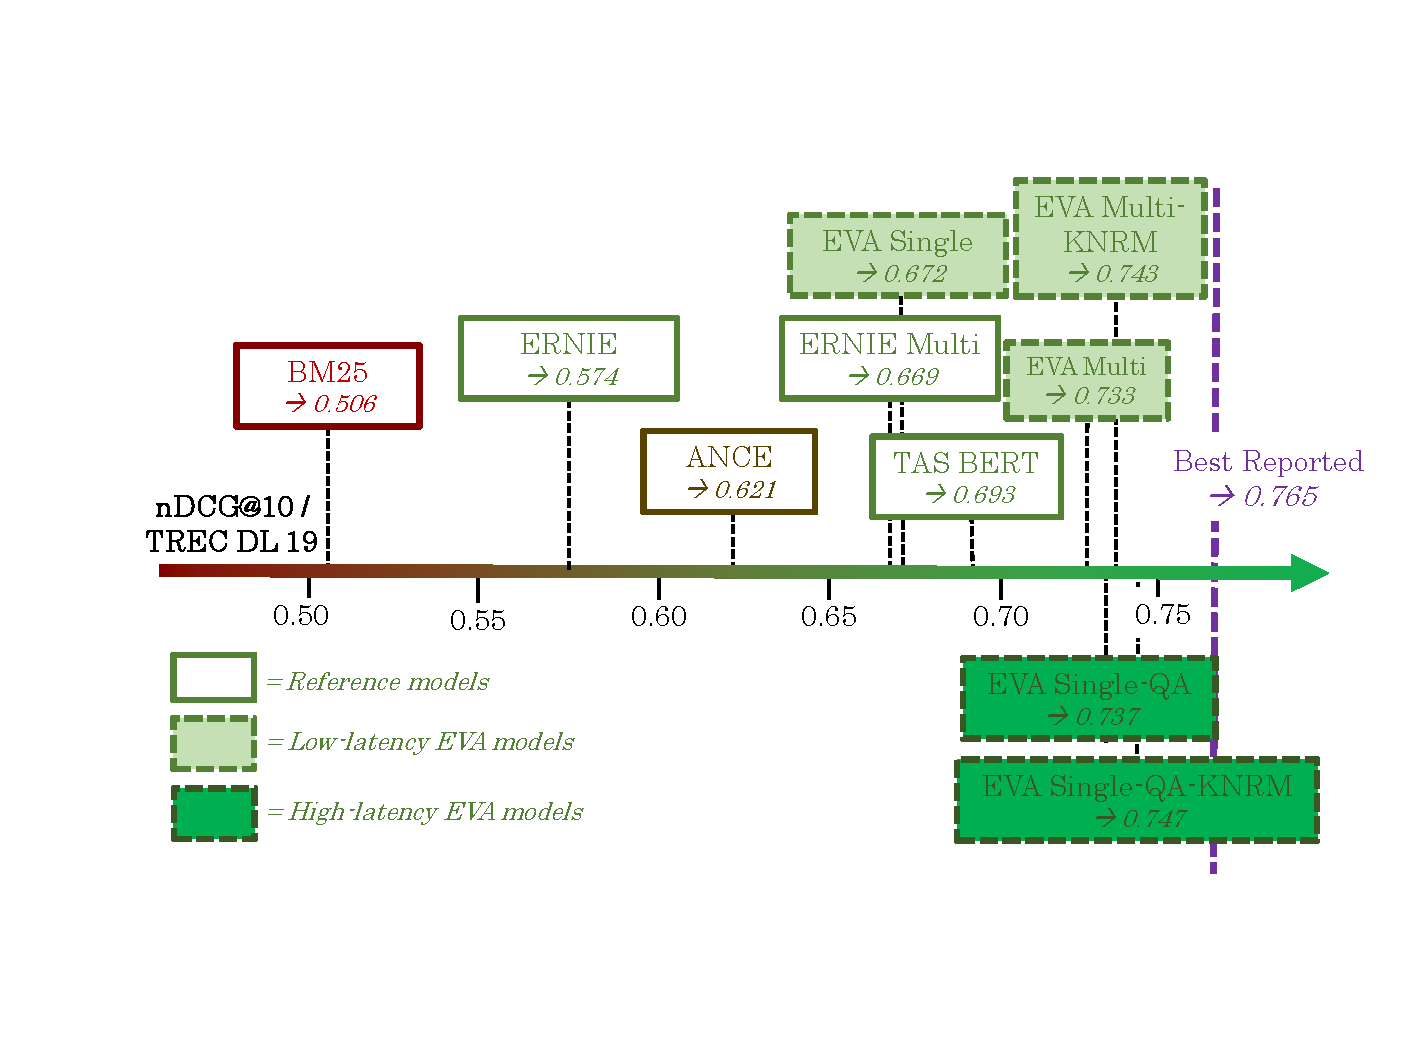
\includegraphics[trim={1.5cm 3cm 0.7cm 3cm}, clip, width=\textwidth]{resources/results} 
    \caption{Exemplary results of EVA models and baselines for TREC DL 19 dataset and evaluation metric nDCG@10}
    \label{fig:results}
\end{figure}

\subsection{Impact}\label{subsec:outcomes}

Based on the results from \autoref{sec:effectiveness} and \autoref{sec:efficiency}, the main outcomes to be attributed to Tran and Yates' work are:
\begin{enumerate}
    \item \textbf{Enriching pre-trained language models with entity embeddings improve effectiveness significantly}:
    The effectiveness results reveal that the models proposed by Tran and Yates, EVA Multi and EVA Single-QA, both with and without KNRM signal, significantly outperform the various baselines. In the given example in \autoref{fig:results}, the value for nDCG@10 of the best performing baseline TAS BERT is 0.693. In contrast, the value for EVA Multi is 0.733, for EVA Single-QA 0.737, which thus corresponds to an increase in effectiveness of 5.8 \% (EVA Multi) and 6.3 \%. Further, the models are only slightly off the best reported results.
    \item \textbf{Multiple entity views increase performance to single view}:
    Considering the performance of the first introduced approach EVA Single, which incorporates entities in documents without a specific focus on the query information, one observes poor results. The EVA Single model even performs worse than the baseline TAS BERT. This is due to the fact that entirely irrelevant entities within documents are taken into account during the retrieval process, thus biasing the results (i.e. see \autoref{subsec:models}). However, if only entities relevant to the respective query are taken into account, which is the case for EVA Single-QA and EVA Multi this leads to a significant increase in effectiveness compared to all baselines, as explained above.
    \item \textbf{KNRM signal provides slight improvement of effectiveness}:
    Comparing the results of the EVA models with additional KNRM signal and without KNRM signal, one observes slightly better results of the EVA models with KNRM signal. This is certainly the case for the example in \autoref{fig:results}, where the EVA Multi KNRM model with an nDCG@10 value of 0.748 is slightly higher than the value of the EVA Multi model of 0.733. The same applies in the setting of the EVA Single-QA model. However, the effect is small; for the TREC DL 2020, the EVA Multi approach even outperforms the same approach with additional KNRM signal. It can be concluded that the impact of introducing entity embeddings is stronger than that of introducing the KNRM signal.
    \item \textbf{Removing known query assumptions has minor impact on effectiveness, but increases efficiency drastically}:
    Best results of effectiveness across all EVA models and baselines are achieved by EVA Multi and EVA Single-QA, as described above. However, the key difference between EVA Multi and EVA Single-QA is the assumption of knowing queries at runtime for EVA Single-QA and the need for large language model inference at runtime (see \autoref{subsec:models}). This leads to large differences in latency compared to the EVA multi-model.. As \autoref{tab:results_effectiveness} shows, the latency for the EVA Multi models is 74 ms with KNRM signal and 76 ms without, while the latency for both of the EVA Single-QA models exceeds two seconds. In a real-world scenario, this would be excessive; users of an information retrieval system do not usually are willing to wait such a long time for results. However, since the effectiveness results of EVA Multi and EVA Single-QA differ only marginally, the EVA Multi approach provides a good trade-off between efficiency and effectiveness.
\end{enumerate}